% GNUPLOT: LaTeX picture with Postscript
\begingroup
  \makeatletter
  \providecommand\color[2][]{%
    \GenericError{(gnuplot) \space\space\space\@spaces}{%
      Package color not loaded in conjunction with
      terminal option `colourtext'%
    }{See the gnuplot documentation for explanation.%
    }{Either use 'blacktext' in gnuplot or load the package
      color.sty in LaTeX.}%
    \renewcommand\color[2][]{}%
  }%
  \providecommand\includegraphics[2][]{%
    \GenericError{(gnuplot) \space\space\space\@spaces}{%
      Package graphicx or graphics not loaded%
    }{See the gnuplot documentation for explanation.%
    }{The gnuplot epslatex terminal needs graphicx.sty or graphics.sty.}%
    \renewcommand\includegraphics[2][]{}%
  }%
  \providecommand\rotatebox[2]{#2}%
  \@ifundefined{ifGPcolor}{%
    \newif\ifGPcolor
    \GPcolortrue
  }{}%
  \@ifundefined{ifGPblacktext}{%
    \newif\ifGPblacktext
    \GPblacktexttrue
  }{}%
  % define a \g@addto@macro without @ in the name:
  \let\gplgaddtomacro\g@addto@macro
  % define empty templates for all commands taking text:
  \gdef\gplbacktext{}%
  \gdef\gplfronttext{}%
  \makeatother
  \ifGPblacktext
    % no textcolor at all
    \def\colorrgb#1{}%
    \def\colorgray#1{}%
  \else
    % gray or color?
    \ifGPcolor
      \def\colorrgb#1{\color[rgb]{#1}}%
      \def\colorgray#1{\color[gray]{#1}}%
      \expandafter\def\csname LTw\endcsname{\color{white}}%
      \expandafter\def\csname LTb\endcsname{\color{black}}%
      \expandafter\def\csname LTa\endcsname{\color{black}}%
      \expandafter\def\csname LT0\endcsname{\color[rgb]{1,0,0}}%
      \expandafter\def\csname LT1\endcsname{\color[rgb]{0,1,0}}%
      \expandafter\def\csname LT2\endcsname{\color[rgb]{0,0,1}}%
      \expandafter\def\csname LT3\endcsname{\color[rgb]{1,0,1}}%
      \expandafter\def\csname LT4\endcsname{\color[rgb]{0,1,1}}%
      \expandafter\def\csname LT5\endcsname{\color[rgb]{1,1,0}}%
      \expandafter\def\csname LT6\endcsname{\color[rgb]{0,0,0}}%
      \expandafter\def\csname LT7\endcsname{\color[rgb]{1,0.3,0}}%
      \expandafter\def\csname LT8\endcsname{\color[rgb]{0.5,0.5,0.5}}%
    \else
      % gray
      \def\colorrgb#1{\color{black}}%
      \def\colorgray#1{\color[gray]{#1}}%
      \expandafter\def\csname LTw\endcsname{\color{white}}%
      \expandafter\def\csname LTb\endcsname{\color{black}}%
      \expandafter\def\csname LTa\endcsname{\color{black}}%
      \expandafter\def\csname LT0\endcsname{\color{black}}%
      \expandafter\def\csname LT1\endcsname{\color{black}}%
      \expandafter\def\csname LT2\endcsname{\color{black}}%
      \expandafter\def\csname LT3\endcsname{\color{black}}%
      \expandafter\def\csname LT4\endcsname{\color{black}}%
      \expandafter\def\csname LT5\endcsname{\color{black}}%
      \expandafter\def\csname LT6\endcsname{\color{black}}%
      \expandafter\def\csname LT7\endcsname{\color{black}}%
      \expandafter\def\csname LT8\endcsname{\color{black}}%
    \fi
  \fi
    \setlength{\unitlength}{0.0500bp}%
    \ifx\gptboxheight\undefined%
      \newlength{\gptboxheight}%
      \newlength{\gptboxwidth}%
      \newsavebox{\gptboxtext}%
    \fi%
    \setlength{\fboxrule}{0.5pt}%
    \setlength{\fboxsep}{1pt}%
    \definecolor{tbcol}{rgb}{1,1,1}%
\begin{picture}(4534.00,3400.00)%
    \gplgaddtomacro\gplbacktext{%
      \csname LTb\endcsname%%
      \put(814,704){\makebox(0,0)[r]{\strut{}$80$}}%
      \csname LTb\endcsname%%
      \put(814,908){\makebox(0,0)[r]{\strut{}$82$}}%
      \csname LTb\endcsname%%
      \put(814,1111){\makebox(0,0)[r]{\strut{}$84$}}%
      \csname LTb\endcsname%%
      \put(814,1315){\makebox(0,0)[r]{\strut{}$86$}}%
      \csname LTb\endcsname%%
      \put(814,1518){\makebox(0,0)[r]{\strut{}$88$}}%
      \csname LTb\endcsname%%
      \put(814,1722){\makebox(0,0)[r]{\strut{}$90$}}%
      \csname LTb\endcsname%%
      \put(814,1925){\makebox(0,0)[r]{\strut{}$92$}}%
      \csname LTb\endcsname%%
      \put(814,2129){\makebox(0,0)[r]{\strut{}$94$}}%
      \csname LTb\endcsname%%
      \put(814,2332){\makebox(0,0)[r]{\strut{}$96$}}%
      \csname LTb\endcsname%%
      \put(814,2536){\makebox(0,0)[r]{\strut{}$98$}}%
      \csname LTb\endcsname%%
      \put(814,2739){\makebox(0,0)[r]{\strut{}$100$}}%
      \csname LTb\endcsname%%
      \put(946,484){\makebox(0,0){\strut{}$0$}}%
      \csname LTb\endcsname%%
      \put(955,484){\makebox(0,0){\strut{}$10000$}}%
      \csname LTb\endcsname%%
      \put(964,484){\makebox(0,0){\strut{}$20000$}}%
      \csname LTb\endcsname%%
      \put(974,484){\makebox(0,0){\strut{}$30000$}}%
      \csname LTb\endcsname%%
      \put(983,484){\makebox(0,0){\strut{}$40000$}}%
      \csname LTb\endcsname%%
      \put(992,484){\makebox(0,0){\strut{}$50000$}}%
      \csname LTb\endcsname%%
      \put(1001,484){\makebox(0,0){\strut{}$60000$}}%
      \csname LTb\endcsname%%
      \put(1010,484){\makebox(0,0){\strut{}$70000$}}%
      \csname LTb\endcsname%%
      \put(1020,484){\makebox(0,0){\strut{}$80000$}}%
      \csname LTb\endcsname%%
      \put(1029,484){\makebox(0,0){\strut{}$90000$}}%
      \csname LTb\endcsname%%
      \put(1038,484){\makebox(0,0){\strut{}$100000$}}%
    }%
    \gplgaddtomacro\gplfronttext{%
      \csname LTb\endcsname%%
      \put(209,1721){\rotatebox{-270}{\makebox(0,0){\strut{}Ocupação (%)}}}%
      \put(992,154){\makebox(0,0){\strut{}Tempo (Coleta)}}%
      \csname LTb\endcsname%%
      \put(3546,2629){\makebox(0,0)[r]{\strut{}sammelt 85}}%
      \csname LTb\endcsname%%
      \put(3546,2409){\makebox(0,0)[r]{\strut{}Arquivo Coleta 90}}%
      \csname LTb\endcsname%%
      \put(3546,2189){\makebox(0,0)[r]{\strut{}Arquivo Coleta 95}}%
      \csname LTb\endcsname%%
      \put(3546,1969){\makebox(0,0)[r]{\strut{}Arquivo Coleta 99}}%
      \csname LTb\endcsname%%
      \put(992,3069){\makebox(0,0){\strut{}Ocupação x Tempo}}%
    }%
    \gplbacktext
    \put(0,0){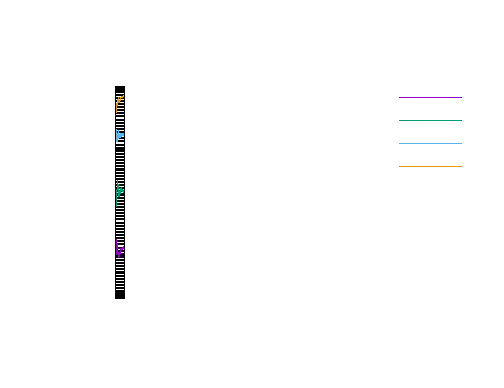
\includegraphics[width={226.70bp},height={170.00bp}]{ocupacao_tempo}}%
    \gplfronttext
  \end{picture}%
\endgroup
